\documentclass{acm_proc_article-sp}
\usepackage{graphicx}
\usepackage{epstopdf}
\usepackage{subfigure}
\usepackage{multirow}
% algorithm package
\usepackage{algorithm}
\usepackage{algorithmic}
\renewcommand{\algorithmicrequire}{ \textbf{Initialization:}}
\renewcommand{\algorithmicensure}{ \textbf{Recurrence:}}

\begin{document}

\title{Datapath Synthesis for Overclocking: Online Arithmetic for Latency-Accuracy Trade-offs}


\numberofauthors{1} %  in this sample file, there are a *total*
% of EIGHT authors. SIX appear on the 'first-page' (for formatting
% reasons) and the remaining two appear in the \additionalauthors section.
%
\author{
% 1st. author
\alignauthor
Authors
%Kan Shi, David Boland and George A. Constantinides\\
%       \affaddr{Department of Electrical and Electronic Engineering}\\
%       \affaddr{Imperial College London}\\
%       \affaddr{London, UK}\\
%       \email{\{k.shi11, david.boland03, g.constantinides\}@imperial.ac.uk}
%\and  % use '\and for second row
}

\maketitle
\begin{abstract}
Digital circuits are currently designed to ensure timing closure. Releasing this constraint by allowing timing violations could lead to significant performance improvements, but conventional forms of computer arithmetic do not fail gracefully when pushed beyond deterministic operation. In this paper we take a fresh look at Online Arithmetic, originally proposed for digit serial operation, and synthesize unrolled digit parallel online operators to allow for graceful degradation. We quantify the impact of timing violation on key arithmetic primitives, and show that substantial performance benefits can be obtained in comparison to binary arithmetic. Since timing errors are caused by long carry chains, these result in errors in least significant digits with online arithmetic, causing less impact than conventional implementations. Using analytical models and empirical FPGA results from an image processing application, we demonstrate an error reduction over 89\% and an improvement in SNR of over 20dB for the same clock rate.
\end{abstract}


% A category with the (minimum) three required fields
\category{H.4}{Information Systems Applications}{Miscellaneous}
%A category including the fourth, optional field follows...
\category{D.2.8}{Software Engineering}{Metrics}[complexity measures, performance measures]

\terms{Design, Performance, Reliability}

\keywords{Online Arithmetic, Overclocking, Imprecise Design, Approximate Computing} % NOT required for Proceedings

\section{Introduction}

\section{Background}
\subsection{Online Arithmetic}
In conventional arithmetic, the computation results are generated either from the least significant digit (LSD), e.g. addition and multiplication, or the most significant digit (MSD), e.g. division and square root. This inconsistency in computing directions would result in large latency when propagating data among different operations. To tackle this problem, online arithmetic has been proposed and studied over the past few decades [xxx]. Both the inputs and outputs are processed in a MSD-first manner using online arithmetic, enabling parallelism among multiple operations. Therefore the overall latency can be largely reduced. Another advantage of online arithmetic is that computations can be dynamically terminated based on the required precision [xxx]. For instance, traditionally $2N$ digits of results will be generated in a $N$-digit multiplier, while only the most significant $N$ digits will be used for successive computations while the $N$ LSDs will be discarded. In contrast, the computation latency can be saved using online arithmetic, which can be finished immediately if the first $N$ digits of results are obtained.

Originally online arithmetic is designed for digit-serial operation. In order to generate the first output digit, $\delta$ digits of inputs are required, as illustrated in Figure xxx. $\delta$ is known as the online delay, which is irrelevant to the precision in a given operation. For ease of discussion, the input to our circuit is normalized to a fixed point number in the range $(-1,1)$. Based on this premise, the online representations of the operands and the results are given by (\ref{Eq:Online_Operands}) [xxx] for $j\in[-\delta,N-1]$.
%
\begin{eqnarray}\label{Eq:Online_Operands}
\footnotesize
  X_{[j]}=\sum_{i=1}^{j+\delta}x_ir^{-i},~Y_{[j]}=\sum_{i=1}^{j+\delta}y_ir^{-i},~Z_{[j]}=\sum_{i=1}^{j}z_ir^{-i}
\normalsize
\end{eqnarray}
%
The MSD-first operation in the online arithmetic is accomplished by utilizing a redundant number system [xxx], in which each digit is represented with a redundant digit set $\{-a,\cdots,-1,0,1,\cdots,a\}$, where $a$ is bounded by $[\frac{r}{2},r-1]$ and $r$ is the radix. Due to the redundancy, the MSDs of the result can be firstly estimated only based on partial information of the inputs and then revised by the following digits.

\subsection{Radix-2 Digit-parallel Online Adder}
Adders serve as a critical building block for arithmetic operations. To perform digit-parallel online addition, the redundant adder can be directly utilized. The adder structure diagram is shown in Figure~\ref{Fig:Radix2SD_adder}. A major advantage with redundant number system over the standard ripple-carry based arithmetic is that the propagation of carry is eliminated, resulting in a precision-independent computation time for addition. As seen in Figure~\ref{Fig:Radix2SD_adder}, the computation delay of this adder is only 2 full adder (FA) delays for any operand word-length, with the cost of one extra FA for each digit of operands Therefore it is unlikely that timing violations happen on the online adder. Due to this reason, this adder structure has been widely used as a part of other arithmetic operators such as multipliers to accelerate the sum of partial products [xxx].
%
\begin{figure}
%\centering
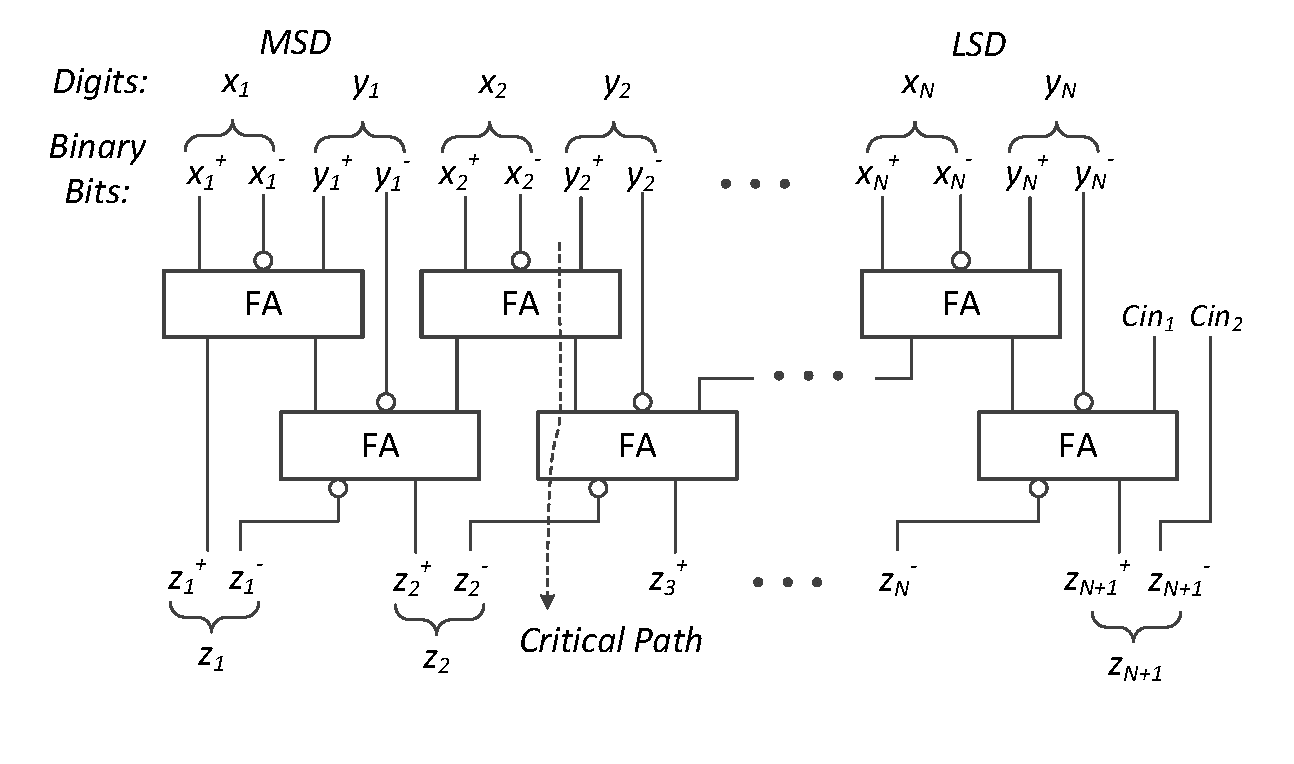
\includegraphics[width=.5\textwidth]{./Figures/SDAdder.pdf}
\vspace{-6.5ex}
\caption{An $N$-digit radix-2 online adder.}
\label{Fig:Radix2SD_adder}
\end{figure}


\section{Online Multiplier}
\subsection{Radix-2 Digit-parallel Online Multiplier}
Multiplication is another key primitive of arithmetic operations. Typically the online multiplication is performed in a recursive manner, as illustrated in Algorithm~\ref{Algorithm:OnlineMult} where both inputs and outputs are $N$-digit number as represented in~(\ref{Eq:Online_Operands}). For a given iteration $j$, the product digit $z_j$ is generated through a selection function $sel()$. In order to ensure the convergence of the algorithm, appropriate selection method and the value of $\delta$ should be determined on the basis of radix $r$ and the digit set. As radix-2 is used most commonly in computer arithmetic, we keep $r=2$ throughout this paper with the corresponding redundant digit set $\{\overline{1},0,1\}$. In this case we have $\delta=3$, and $sel()$ is given by (\ref{Eq:SelFunc_OM})[xxx]. It can be seen that the decision is made only based on 1 integer bit and 1 fractional bit of $W_{[j]}$.
%
\begin{algorithm}[tbp]
  \caption{Online Multiplication}
  \begin{algorithmic}[1]
    \REQUIRE~$X_{[-\delta]}=Y_{[-\delta]}=P_{[-\delta]}=0$
    \ENSURE~$for~~ j=-\delta,~-\delta+1,~\cdots,~N-1 ~~do$
      \begin{eqnarray}\label{Eq:OnlineMult_General}
        \begin{matrix}
          H_{[j]}   & = & r^{-\delta}\left(x_{j+\delta+1}\cdot Y_{[j+1]}+y_{j+\delta+1}\cdot X_{[j]}\right)\\
          W_{[j]}   & = & P_{[j]} + H_{[j]}\\
          z_j       & = & sel(W_{[j]})\\
          P_{[j+1]} & = & r\left(W_{[j]}-z_j\right)
        \end{matrix}
      \end{eqnarray}
  \label{Algorithm:OnlineMult}
  \end{algorithmic}
\end{algorithm}
%
\begin{eqnarray}\label{Eq:SelFunc_OM}
  sel(W_{[j]})=\begin{cases}
    1 & \text{ if } W_{[j]} \geqslant \frac{1}{2} \\
    0 & \text{ if } -\frac{1}{2}\leqslant W_{[j]}<\frac{1}{2} \\
    \overline{1} & \text{ if } W_{[j]}<-\frac{1}{2}
  \end{cases}
\end{eqnarray}
%
%
\begin{figure}[tbp]
\centering
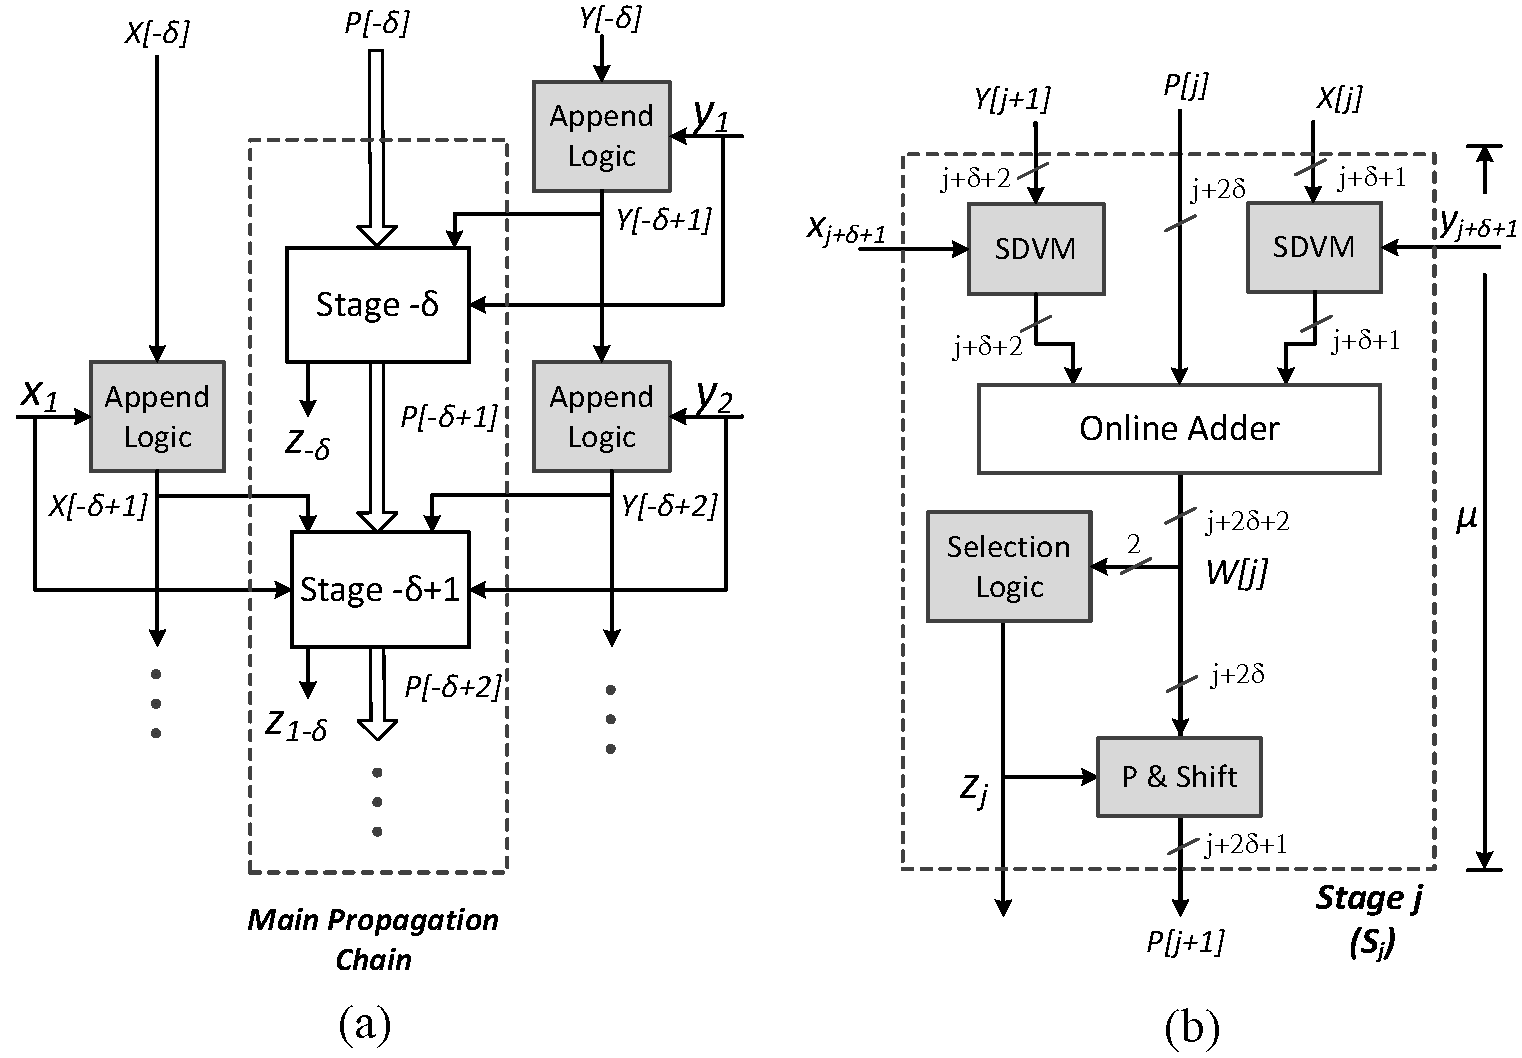
\includegraphics[width=.49\textwidth]{./Figures/OnlineMult_Unrolled.pdf}
\vspace{-3ex}
\caption{(a) Synthesis of Algorithm 1 into a digit-parallel online multiplier (b) Structure of one stage.}
\label{Fig:Radix2OnlineMultiplier}
\end{figure}

Algorithm \ref{Algorithm:OnlineMult} can be synthesized into a unrolled digit parallel structure as shown in  Figure~\ref{Fig:Radix2OnlineMultiplier}(a). In an $N$-digit OM, there are totally $N+\delta$ stages, of which the online inputs are generated from the appending logic according to (\ref{Eq:Online_Operands}). For each stage, an online adder is used as shown in Figure~\ref{Fig:Radix2OnlineMultiplier}(b). The SDVM module performs the signed-digit vector multiplication. When $r=2$ and the digit set $\{\overline{1},0,1\}$ is used, the implementation of SDVM is straight forward, because for instance the output of $(y_{j+\delta+1}\cdot X_{[j]})$ is 0, $X_{[j]}$ or $-X_{[j]}$ when $y$ equals to $0$, $1$ and $-1$ respectively.

Instead of duplicating the digit-serial implementation $N+\delta$ times, each stage in the digit-parallel architecture can be optimized for area reduction. For instance, the SDVM modules and the appending logic are not required in the last $\delta$ stages because the inputs are 0. This leads to a smaller online adder in these stages. Similarly for the first $\delta$ stages the selection logic can be removed, as the first digit of the result is generated at $S_0$.

\subsection{Analysis of The Critical Path}

From Figure \ref{Fig:Radix2OnlineMultiplier} we observe two types of delay chains. One is caused by generation and propagation of $P_{[j]}$ among different stages. The other is the generation of online inputs from the appending logic. Since the appending logic is basically wires, the overall latency will eventually be determined by the delay from the first source, especially with increasing operand word-lengths. As such, we initially model the delay of each stage within an online multiplier to be a constant value $\mu$. We also assume that the generation of online inputs costs no delay.

For an $N$-digit OM, let a propagation chain is generated at $S_{\tau}$ with the length of $d(\tau)$ digits, then $\tau$ is bounded by (\ref{Eq:Bound_GenChain}).
%
\begin{eqnarray}\label{Eq:Bound_GenChain}
  -\delta\leqslant\tau\leqslant N-1-\delta
\end{eqnarray}
%
Suppose a chain is generated at the first stage $S_{-\delta}$ and is propagated to the final stage $S_{N-1}$. This corresponds to $d(\tau)=N+\delta$ and hence the critical path delay of the OM is then given by (\ref{Eq:WorstCaseDelay_NaiveAnalysis}). Note that this value is normally employed by the timing analysis tools together with a guard-band to ensure a correct functionality across a variety of operating conditions.
%
\begin{eqnarray}\label{Eq:WorstCaseDelay_NaiveAnalysis}
  \mu_{OM\_structural} = (N+\delta)\cdot \mu
\end{eqnarray}
%
For a given stage $S_\tau$ when inputs are initially introduced, we have $W_{[\tau]}=H_{[\tau]}$ as $P_{[\tau]}=0$. From (\ref{Eq:OnlineMult_General}) the maximum word-length of $H_{[\tau]}$ and $P_{[\tau]}$ is $(\tau+2\delta+2)$ and $(\tau+2\delta)$, respectively. Thus the propagation of $P_{[\tau]}$ will only affect the first $(\tau+2\delta)$ MSDs of $W_{[\tau]}$. As an example, the maximum word-length of $P_{[-2]}$ is 4 digits while the value of $H_{[-2]}$ is 6. After delay $\mu$ from the start of computation, only the first 4 digits of $W_{[-2]}$ will be changed by the propagation of $P_{[-2]}$, as labeled on the segment of $P_{[-2]}$ in Figure~\ref{Fig:TimingGraph_OM}. During each propagation, this value is reduced by 1 due to the shifting to derive $P_{[j+1]}$ in (\ref{Eq:OnlineMult_General}). Finally this chain annihilates if the number shrinks to 1, because for all possible changes as listed in Table~\ref{Tab:Annihilation}, the propagation output keeps unchanged. In the previous example, the chain generated at $S_{-3}$ will annihilate at $S_1$ as shown in Figure \ref{Fig:TimingGraph_OM}. Besides, chains generated at other stages with the maximum lengths are also depicted for a 3-digit OM. It can be seen that the actual worst-case delay is $5\mu$, instead of $6\mu$ as predicted by (\ref{Eq:WorstCaseDelay_NaiveAnalysis}).
%
\begin{figure}[tbp]
\centering
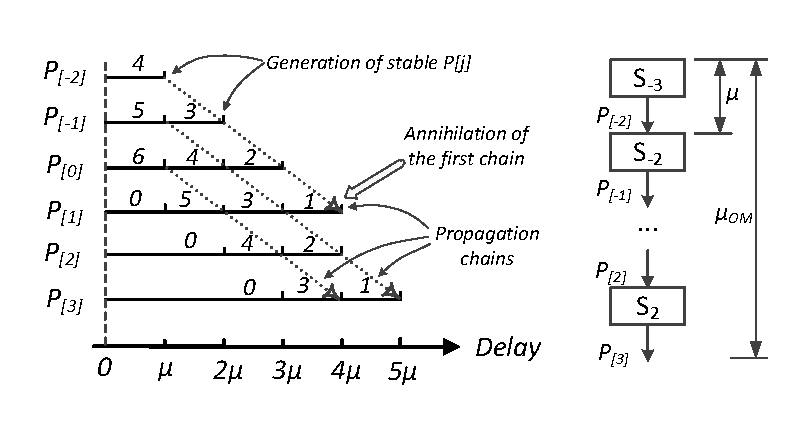
\includegraphics[width=.5\textwidth]{./Figures/Timing_3DigitOM.pdf}
\vspace{-5ex}
\caption{All possible chains with the maximum length in a 3-digit online multiplier. The numbers on the line segment represent the number of the updated MSDs of $W_{[j]}$.}
\label{Fig:TimingGraph_OM}
\end{figure}
%
\begin{table}[tbp]
\centering
\caption{All the combinations of ${W}_{[j]}$ of which 2 MSBs might change. Together with the corresponding $z_j$ and the integer bit of $P_{[j+1]}$.}
\begin{tabular}{|c|c|c|c|}
\hline
${W}_{[j]}$&$z_j$&$P_{[j+1]}=2(W_{[j]}-z_j)$\\ \hline
 $0.0\rightarrow1.0$ & $0\rightarrow\overline{1}$ & $0\rightarrow0$\\ \hline
 $0.1\rightarrow1.1$ & $1\rightarrow0$ & $1\rightarrow1$\\ \hline
 $1.0\rightarrow0.0$ & $\overline{1}\rightarrow0$ & $0\rightarrow0$\\ \hline
 $1.1\rightarrow0.1$ & $0\rightarrow{1}$ & $1\rightarrow1$\\  \hline
\end{tabular}
\label{Tab:Annihilation}
\vspace{-2ex}
\end{table}

In general for a given value of $\tau$, the maximum value of $d(\tau)$ is bounded by two constraints. On one hand, the chain length cannot be greater than $N-1$. On the other hand, the altered digit number of $P_{[\tau+1]}$ will eventually reduced to 1. The combination of both gives (\ref{Eq:Bound_ChainLength}).
%
\begin{eqnarray}\label{Eq:Bound_ChainLength}
  d(\tau)_{max}=Min(N-1-\tau,~\tau+2\delta+1)
\end{eqnarray}
For all values of $\tau$ in (\ref{Eq:Bound_GenChain}), the critical path delay of the OM is then given by (\ref{Eq:MaxChainLength_OneStage}).
%
\begin{eqnarray}\label{Eq:MaxChainLength_OneStage}
  \mu_{OM}=Max(d(\tau)_{max})\cdot\mu
\end{eqnarray}
%
Substituting (\ref{Eq:Bound_GenChain}) and (\ref{Eq:Bound_ChainLength}) into (\ref{Eq:MaxChainLength_OneStage}), we obtain the expression of $\mu_{OM}$ in (\ref{Eq:WorstCaseDelay_OM}). The comparison between (\ref{Eq:WorstCaseDelay_NaiveAnalysis}) and (\ref{Eq:WorstCaseDelay_OM}) is illustrated in Figure \ref{Fig:Gap_OM}, from which we see that the OM could run at a higher frequency than predicted from naive structural timing analysis.
%
\begin{eqnarray}\label{Eq:WorstCaseDelay_OM}
  \mu_{OM} = \begin{cases}
    \frac{N-1}{2}\cdot\mu+4\mu & \text{if N is odd}\\
    \frac{N-2}{2}\cdot\mu+4\mu & \text{if N is even}
  \end{cases}
\end{eqnarray}

%
\begin{figure}[t]
    \centering
    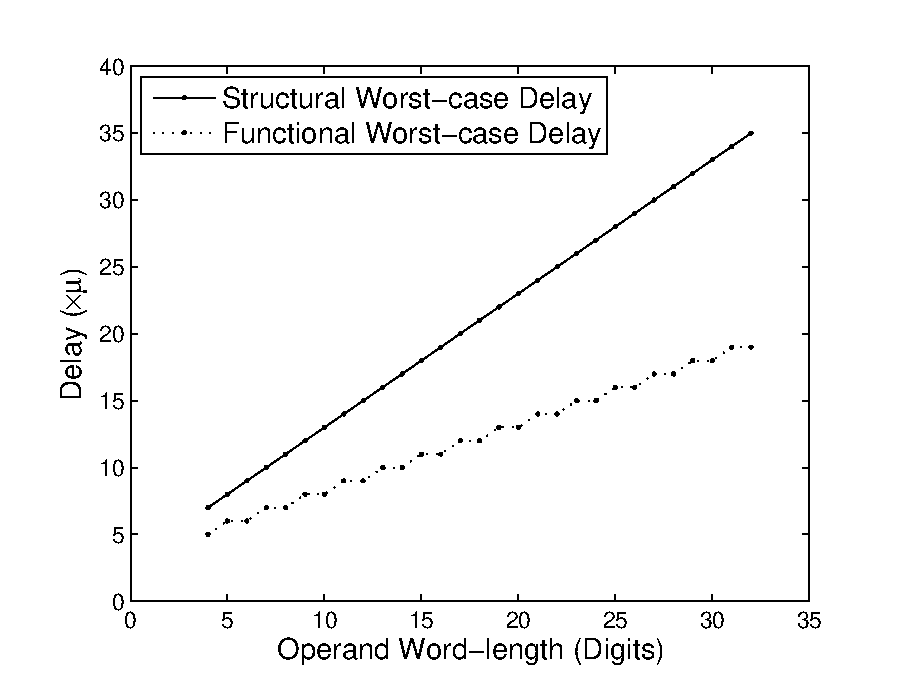
\includegraphics[width=.4\textwidth]{./Figures/Gap.eps}
    %\vspace{-5ex}
    \caption{Comparison between the worst-case delay of an online multiplier obtained from (\ref{Eq:WorstCaseDelay_NaiveAnalysis}) and (\ref{Eq:WorstCaseDelay_OM}).}
\label{Fig:Gap_OM}
\end{figure}


\subsection{Probabilistic Model of Overclocking \\Error}
For an $N$-digit OM, it follows that if the sampling period $T_S$ is greater than $\mu_{OM}$, correct results will be sampled. If, however, faster-than-rated sampling frequencies are applied such that $T_S<\mu_{OM}$, timing violations might happen and intermediate results will be sampled, potentially generating errors. For a given $T_S$, the maximum length of error-free propagation is described by (\ref{Eq:MaxChainLength}) where $f_S$ denotes the sampling frequency. We assume that the first digit of the result will be generated correctly, i.e. $b>3$. The upper bound of parameter $\tau$ in (\ref{Eq:Bound_GenChain}) is then modified as given by (\ref{Eq:UppBoundofChainNo}). In this Section, we model the probability and the magnitude of the overclocking error, under the assumption that every digit of each input to our circuit is uniformly and independently generated with the digit set $\{\overline{1},0,1\}$. Nevertheless, the assumption will be relaxed in Section xxx where real image data are used.
%
\begin{eqnarray}\label{Eq:MaxChainLength}
  b:=\left\lceil \frac{T_S}{\mu} \right\rceil=\left\lceil \frac{1}{\mu\cdot f_S}\right\rceil
\end{eqnarray}
%
%
\begin{eqnarray}\label{Eq:UppBoundofChainNo}
  \tau\leqslant N-1-b=\tau_{upp}
\end{eqnarray}

\subsubsection{Probability of Timing Violations}
If a chain is generated at $S_{\tau}$, the presence of timing violation requires $d(\tau)>b$. Since the propagation and annihilation of the chain in an OM is irrelevant to the operand word-length, the probability of $d(\tau)$ is only dependent upon the specific input pattern of $S_{\tau}$, which is denoted as $C(\tau)$. In general there are four types of inputs as listed in (\ref{Eq:AllInputCases}). Under the assumption that all digits of input signal are mutually independent, the probability of $C_1\sim C_4$ equal to $4/9$, $1/9$, $2/9$ and $2/9$ respectively.
%
\begin{eqnarray}\label{Eq:AllInputCases}
  C(\tau)=\left\{\begin{matrix}
    \text{Case 1~(}C_1{):} & x_{\tau+\delta+1}\neq0,~y_{\tau+\delta+1}\neq0\\
    \text{Case 2~(}C_2{):} & x_{\tau+\delta+1}=0,~y_{\tau+\delta+1}=0\\
    \text{Case 3~(}C_3{):} & x_{\tau+\delta+1}\neq0,~y_{\tau+\delta+1}=0\\
    \text{Case 4~(}C_4{):} & x_{\tau+\delta+1}=0,~y_{\tau+\delta+1}\neq0
  \end{matrix}\right.
\end{eqnarray}
%
As discussed when deriving (\ref{Eq:Bound_ChainLength}), the value of $d(\tau)$ corresponds to the word-length of $P_{[\tau+1]}$ when computation initially starts. That is, (\ref{Eq:OnlineMult_General}) can be modified to give (\ref{Eq:P_Wordlength}) for $\tau>-\delta$. Therefore the word-length of $P_{[\tau+1]}$ is best considered separately for different value of $C(\tau)$.
\begin{eqnarray}\label{Eq:P_Wordlength}
  \begin{aligned}
    P_{[\tau+1]} &= r\cdot W_{[\tau]}\\
                 &= r^{-\delta+1}(x_{\tau+\delta+1}Y_{[\tau+1]}+y_{\tau+\delta+1}X_{[\tau]})\\
  \end{aligned}
\end{eqnarray}
%
If $C(\tau)=C_1$, $P_{[\tau+1]}$ embodies the maximum word-length and hence $d(\tau)=d(\tau)_{max}$ as given in (\ref{Eq:MaxChainLength_OneStage}). If $C(\tau)=C_2$, we have $P_{[\tau+1]}=0$. In this case no chain is generated and $d(\tau)=0$. Similarly the probability is $1/9$.

Since $C_3$ and $C_4$ are statistically identical, we only discuss the situation that $C(\tau)=C_3$. In this case the word-length of $P_{[\tau+1]}$ only depends on that of $Y_{[\tau+1]}$. Besides, we have $Y_{[\tau+1]}=Y_{[\tau]}$. It means $d(\tau)$ becomes dependent of the inputs of previous stage $S_{\tau-1}$. There are 2 possible situations for $\tau>-\delta$ as stated below:
\vspace{-1ex}
\begin{itemize}
  \item For the previous stage if $y_{\tau+\delta}\neq0$, then the word-length of $Y_{[\tau]}$ is maximized. Thus $d(\tau)=d(\tau)_{max}-1$.
  \item If $y_{\tau+\delta}=0$, then $Y_{[\tau]}=Y_{[\tau-1]}$. This is a recursive process and these two judgements will be performed again for $\tau=\tau-1$. It terminates when $\tau=-\delta$ or the first judgement is satisfied.
\end{itemize}
\vspace{-1ex}
For the first stage where $\tau=-\delta$, (\ref{Eq:P_Wordlength}) can be modified further yielding $P_{[-\delta+1]}=r^{\delta+1}(x_1Y_{[-\delta+1]})$. Therefore the value in (\ref{Eq:MaxChainLength_OneStage}) can only be achieved when $C(-\delta)=C_1$, otherwise $d(-\delta)=0$.

In summary, we derive Algorithm 2 to go through all possible stages that timing violations may occur and the corresponding inputs. This algorithm returns $Prob(T_S)$, which denotes the probability that timing violations happen in an $N$-digit online multiplier under a given $T_S$. $Prob(i,C(i))$ denotes the probability of the input pattern for stage $i$.
%
\begin{algorithm}[htbp]
  \caption{Probability of Timing Violations}
  \begin{algorithmic}[1]
    \STATE  $Prob(T_S)=0$
    \FORALL {stages $\tau\in\{-\delta,-\delta+1,\cdots,\tau_{upp}\}$ and input cases $C(\tau)\in\{C_1,\cdots,C4\}$}
    \STATE  Determine $d(\tau)$ based on $C(\tau)$
    \IF     {$d(\tau)>b$}
    \STATE  $Prob(T_S)=Prob(T_S)+\prod_{i=-\delta}^{\tau}Prob(i,C(i))$
    \ENDIF
    \ENDFOR
    \RETURN $Prob(T_S)$
  \label{Algorithm:ProbabilityTimingViolation}
  \end{algorithmic}
\end{algorithm}

\subsubsection{Magnitude of Overclocking Error}
For a given $T_S$, timing violations may happen on multiple chains. For instance in Figure~\ref{Fig:TimingGraph_OM} if $T_S=3.5\mu$, all the 3 chains would not be correctly propagated and all the three digits of the outputs are affected. For the first chain that timing violation may occur, i.e. $d(\tau)_{max}>b$, let it annihilate at annihilate at $S_{\lambda}$ where $\lambda=\tau+d_{max}(\tau)-1$. Therefore overclocking errors may happen from digit $\lambda$ to digit $N-1$ of the product. In general the magnitude of overclocking error is given by (\ref{Eq:ErrorMagnitude}), where $z_i$ and ${z_i}'$ denote the correct value and the actual value of the output digit of $S_i$, separately.
%
\begin{eqnarray}\label{Eq:ErrorMagnitude}
\scriptsize
  \left|\varepsilon\right|=\left|\sum_{i=\lambda}^{N-1}2^{-i-1}(z_i-{z_i}')\right|=\left|\sum_{i=\lambda}^{N-1} \varepsilon_i\right|
\normalsize
\end{eqnarray}
%
However, the change of output digits might not result in a new number with online arithmetic, because of the redundancy in number representation. For instance, the two's complement number $0.111$ can be represented in the online form as $0.10\overline{1}$, $0.1\overline{1}1$ and $0.111$.

Specifically as seen in Figure \ref{Fig:TimingGraph_OM}, only the MSD of ${W}_{[\lambda]}$ will change during ${z_\lambda}'\rightarrow z_\lambda$. Therefore $\Delta z_i=z_i-{z_i}'$ could be $\pm1$ according to Table \ref{Tab:Annihilation}. Whereas in other cases, ${W}_{[i]}$ might change 2 MSDs, potentially results in errors being $0$, $\pm1$ and $\pm2$.

Now we notice that the overclocking error is not a deterministic value for a given $T_S$. Thus instead of directly using (\ref{Eq:ErrorMagnitude}), we employ the expectation of error magnitude across these variations on the condition of the appearance of timing violations as given by (\ref{Eq:Error_Overclocking}) where $\varepsilon_\lambda=\pm2^{-\lambda-1}$ and $\varepsilon_i\in\{0,\pm2^{-i-1},\pm2^{-i}\}$.
%
\begin{eqnarray}\label{Eq:Error_Overclocking}
\scriptsize
      E(|\varepsilon|)=E\left(\left|\varepsilon_\lambda+\sum_{i=\lambda+1}^{N-1}\varepsilon_i \right|\right)
\normalsize
\end{eqnarray}

\subsubsection{Expectation of Overclocking Error}
For a given $T_S$, the combination of $Prob(T_S)$ and $E(|\varepsilon|)$ in Algorithm 2 and (\ref{Eq:Error_Overclocking}) yields the overall expectation of overclocking error, as presented in (\ref{Eq:Expectation_Overclocking}). The verification of the proposed model is illustrated in Figure \ref{Fig:ModelVerification} against the results from Monte-Carlo simulations based on the aforementioned timing model. $T_S$ is normalized with respect to the value from (\ref{Eq:WorstCaseDelay_NaiveAnalysis}). Note that both results are obtained when assuming the input data are randomly generated following uniform distribution. It can be seen that the modeled value match well with the simulation results.
%
\begin{eqnarray}\label{Eq:Expectation_Overclocking}
  E_{ovc}=Prob(T_S)\cdot E(|\varepsilon|)
\end{eqnarray}

\begin{figure}[t]
  %\vspace{-2ex}
  \centering
  %\vspace{-4ex}
  \subfigure[8-digit]{
  \begin{minipage}{0.24\textwidth}
    %\centering
    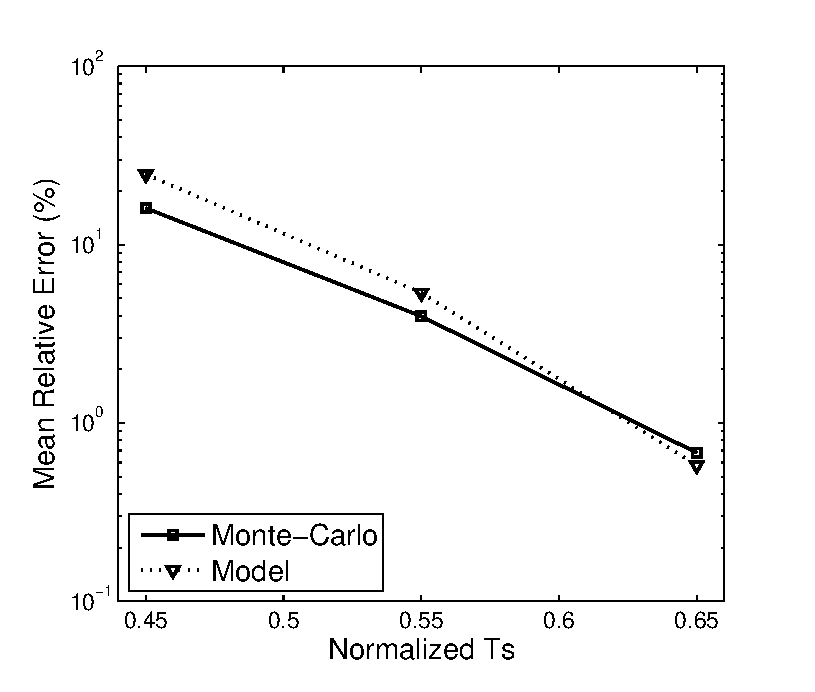
\includegraphics[width=1.7in]{./Figures/WL8_Model.eps}
  \end{minipage}%
  }% This is important! use % to indicate same line, otherwise new line
  \subfigure[12-digit]{
  \begin{minipage}{0.24\textwidth}
    %\centering
    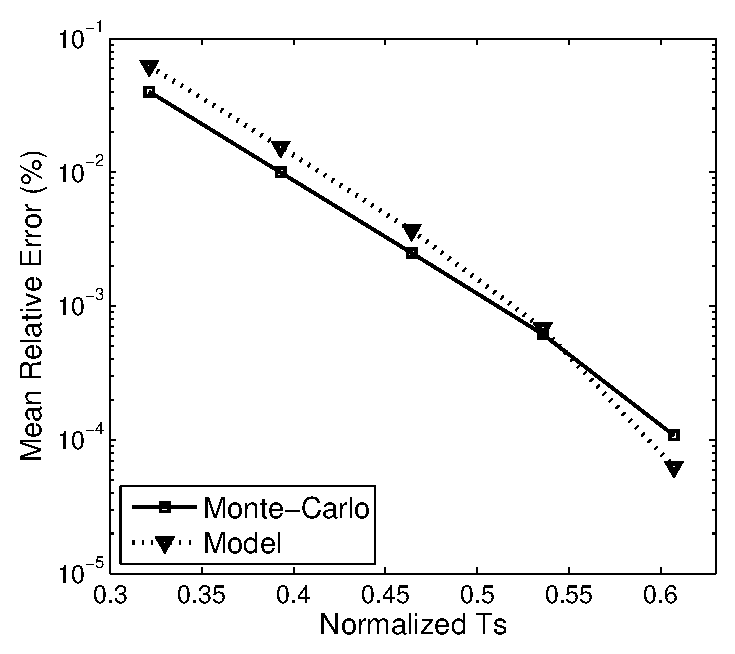
\includegraphics[width=1.7in]{./Figures/WL12_Model.eps}
  \end{minipage}
  }
  \vspace{-2ex}
  \caption{Expectation of overclocking error for online multipliers: verification of the proposed model against Monte-Carlo simulations based on aforementioned timing models.}
  \label{Fig:ModelVerification}
  \vspace{-2ex}
\end{figure}

For all possible $\tau$ as bounded by (\ref{Eq:Bound_GenChain}), the probability of different chain lengths within an $N$-digit OM and the corresponding magnitude of overclocking error can be obtained, as shown in Figure \ref{Fig:Probability_Error_Mean} with $N=8,12,16,32$, respectively. For a given $T_S$, the overall expectation of overclocking error in (\ref{Eq:Expectation_Overclocking}) can also be computed by (\ref{Eq:PDF_MeanError}).
%
\begin{eqnarray}\label{Eq:PDF_MeanError}
  E_{ovc}=\sum_{d>b}P_d\cdot\varepsilon_d
\end{eqnarray}
%
From Figure \ref{Fig:Probability_Error_Mean} several observations can be made. First, the error magnitude decreases exponentially with longer chain lengths, because in contrast to the conventional arithmetic, timing violation firstly affects LSDs with online arithmetic. Second, chains with longer delay would happen with greater probabilities in an OM, because the delay is mainly dependent upon the inputs that generate the chain, while the chain propagation and annihilation will not be affected by the inputs. For the traditional ripple-carry-based arithmetic, specific input patterns are required to decide carry generation, propagation and annihilation. In addition, carry chains could not be overlapped with traditional arithmetic, whereas long chains might occur simultaneously and mutually overlapped within the OM, as shown previously in Figure \ref{Fig:TimingGraph_OM}. However, we also notice that for chains with long delays, the increasing speed of probability is much slower than the decreasing speed of error magnitude with long chain delays. Therefore the combination of both would results in a decline in error expectation. In traditional arithmetic, the decrease of probability is offset by the growth of error magnitude, as both of them vary exponentially. Hence the error expectation with respect to each chain delay keeps almost constant. This finding indicates that the OM is less sensitive to overclocking error than the multiplier using traditional arithmetic, especially when timing violations initially appear.

\begin{figure}[t]
  %\vspace{-2ex}
  \centering
  \subfigure[8-digit]{
  \begin{minipage}{0.24\textwidth}
    %\centering
    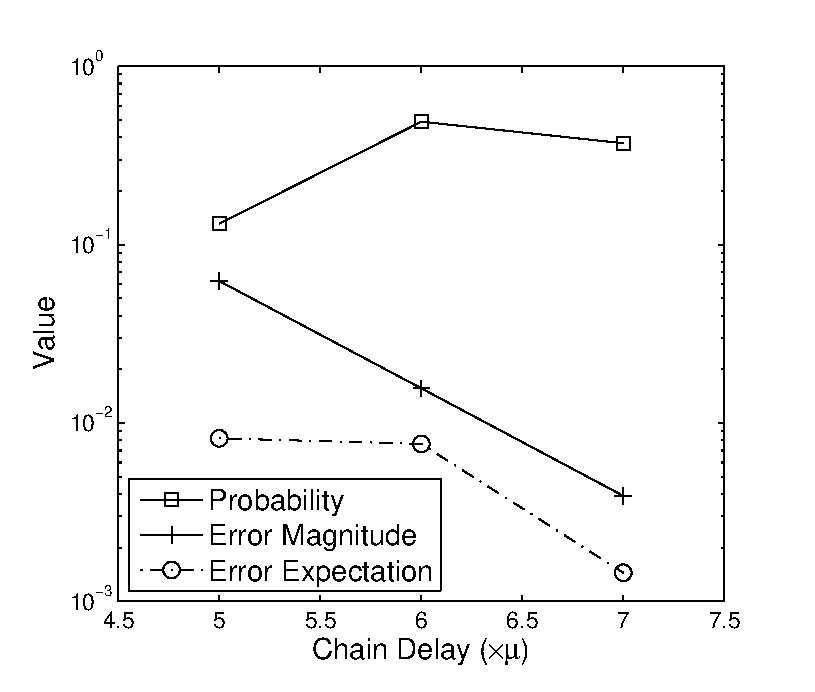
\includegraphics[width=1.7in]{./Figures/PE8.eps}
  \end{minipage}%
  }% This is important! use % to indicate same line, otherwise new line
  \subfigure[12-digit]{
  \begin{minipage}{0.24\textwidth}
    %\centering
    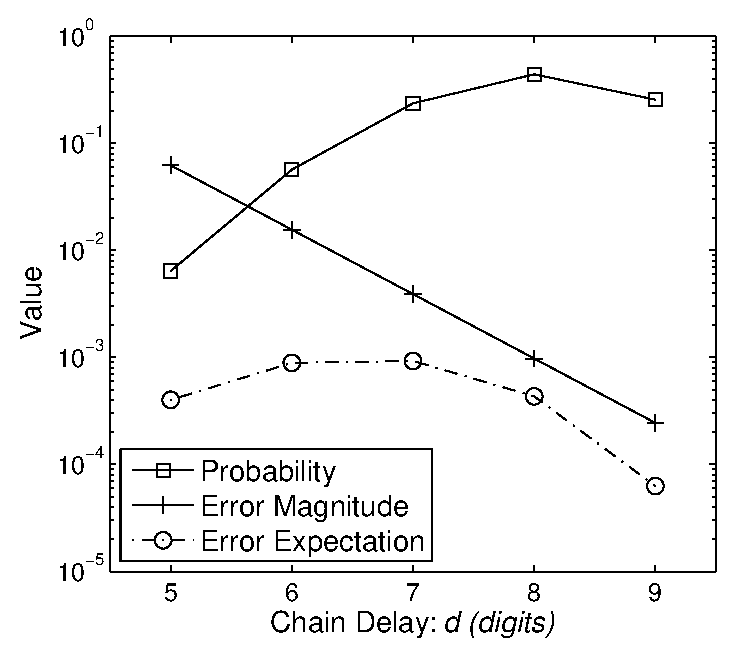
\includegraphics[width=1.7in]{./Figures/PE12.eps}
  \end{minipage}
  }\vspace{-2ex}
  \subfigure[16-digit]{
  \begin{minipage}{0.24\textwidth}
    %\centering
    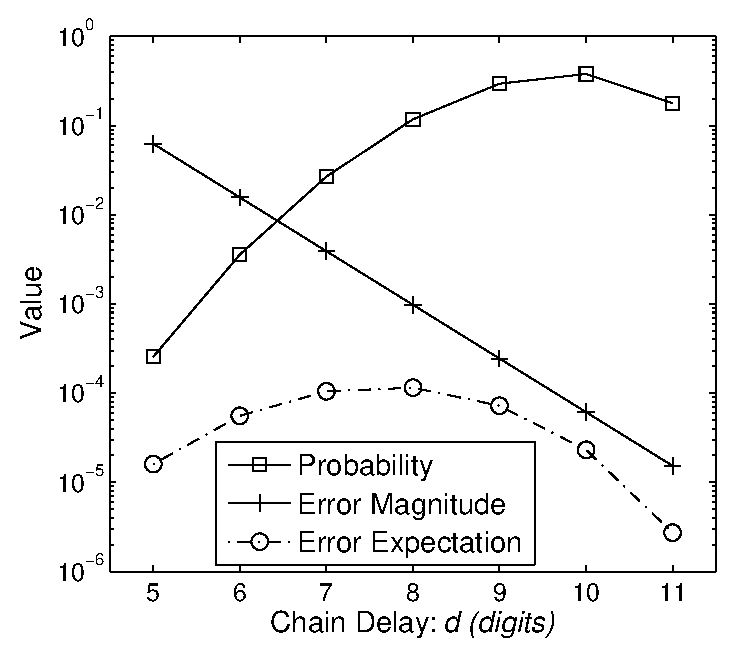
\includegraphics[width=1.7in]{./Figures/PE16.eps}
  \end{minipage}%
  }% This is important! use % to indicate same line, otherwise new line
  \subfigure[32-digit]{
  \begin{minipage}{0.24\textwidth}
    %\centering
    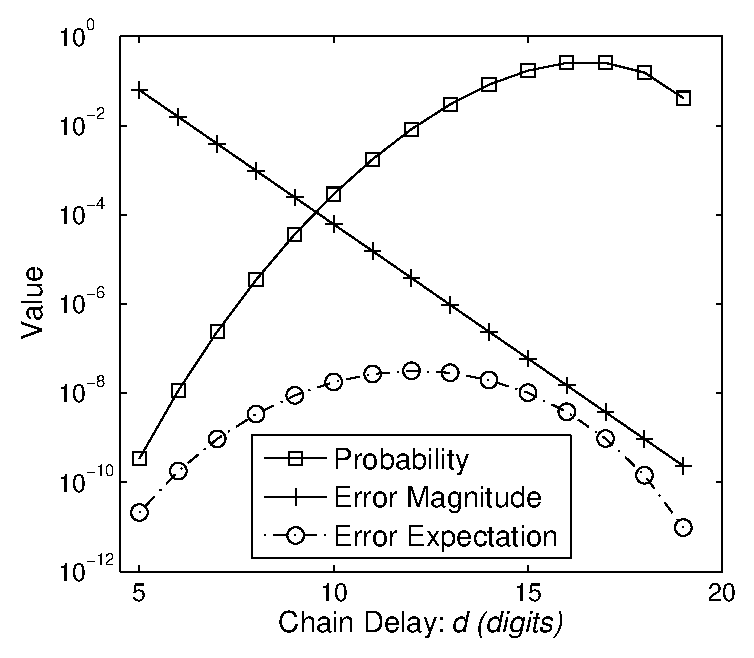
\includegraphics[width=1.7in]{./Figures/PE32.eps}
  \end{minipage}
  }
  \vspace{-3ex}
  \caption{Probabilities of different chain delay, the corresponding magnitude of overclocking error and the combination of both in terms of error expectation in a radix-2 OM.}
  \label{Fig:Probability_Error_Mean}
  \vspace{-2ex}
\end{figure}

\section{Case Study: Image Filter}
\subsection{Experimental Setup}
The benefits of the proposed methodology are demonstrated by using a Gaussian image filter, which is implemented using two types of computer arithmetic. One is the radix-2 traditional arithmetic and data are represented in the 2's complemented form. In this case, adders and multipliers are created using Xilinx Core Generator[xxx] with speed optimization. The other is the radix-2 online arithmetic, of which basic building blocks are described in previous sections. In this case, all inputs and outputs are represented in the online format. In order to achieve the desired latency between input and output, both designs are overclocked and the error seen at the output are recorded. The results are obtained from a Xilinx Virtex-6 FPGA through post place-and-route simulations. In our experiments, the results are evaluated in terms of mean relative error (MRE), which represents the percentage of error at outputs, as given by (\ref{Eq:MRE}) where $E_{error}$ and $E_{out}$ refer to the mean value of error and correct output, respectively.
%
\begin{eqnarray}\label{Eq:MRE}
  MRE=\left|\frac{E_{error}}{E_{out}}\right|\times100\%
\end{eqnarray}
%
Since the redundant digit set is used in online arithmetic, a signed integer number within $[-2^N,2^N-1]$ can be represented using $N$ digits. However the representation range is $[-(2^{N-1},2^{N-1}-1)]$ with $N$ digits using 2's complement number system. For a valid comparison, an $N$-digit image filter using online arithmetic is employed against an $(N+1)$-digit design using traditional arithmetic. In our experiments, two types of input data are utilized. One is randomly sampled from a uniform distribution of $N$-digit numbers. This type is referred to as ``Uniform Independent (UI) inputs''. The other is called ``real inputs'', which are the pixel values of several benchmark images.

\subsection{Impact of Overclocking on Different\\ Arithmetic}
The values of overclocking error of the image filter based on traditional arithmetic (dotted lines) and online arithmetic (solid lines) when $N=8$ are illustrated in Figure \ref{Fig:MRE_ImageFilter}. According to the timing analysis tool, the rated operating frequencies of the two designs are $168.7$MHz and $148.3$MHz, respectively. However as seen in Figure \ref{Fig:MRE_ImageFilter}, for both input types the online image filter actually operates at a higher frequency without timing violations in comparison to the design using traditional arithmetic, as predicted in Section xxx. In addition, this error-free frequency is even larger when using the real image data as inputs, since the real data do not exactly follow the uniform distribution or the independent assumption. In Figure \ref{Fig:MRE_ImageFilter} the real inputs are the results for the ``Lena'' benchmark image.
%
\begin{figure}
    \centering
    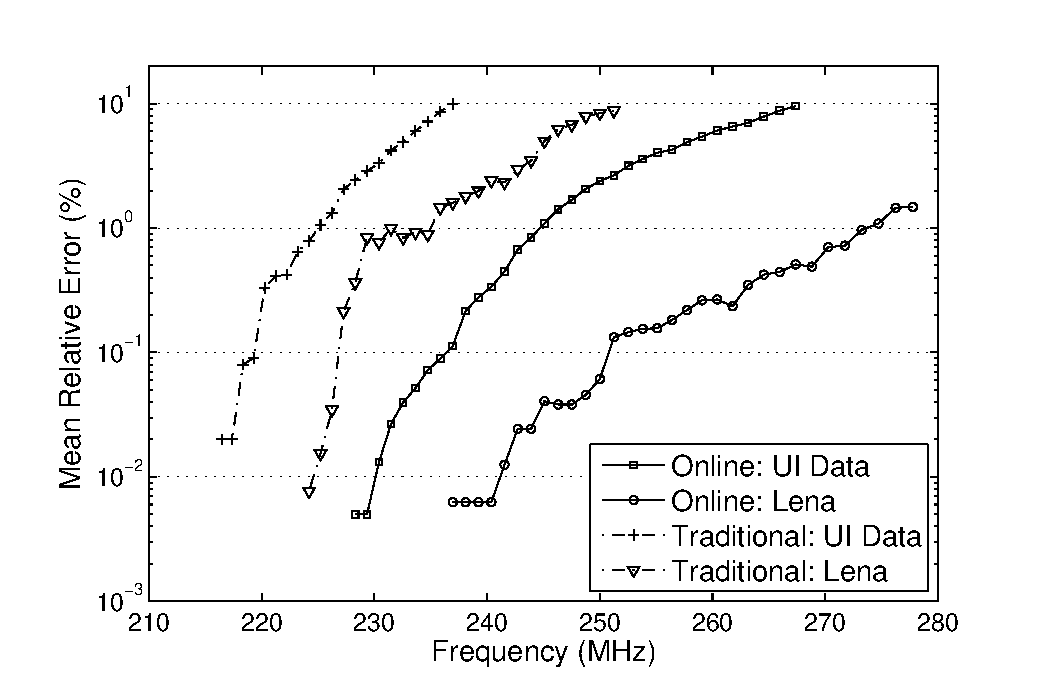
\includegraphics[width=.5\textwidth]{./Figures/MRE.eps}
    \caption{Overclocking error in an image filter with two types of computer arithmetic: online arithmetic and standard binary arithmetic, of which the rated frequencies are 148.3MHz and 168.7MHz, respectively, according to the timing analysis tool.}
\label{Fig:MRE_ImageFilter}
\end{figure}

%\subsection{Sensitivity of Overclocking Error}
If errors can be tolerated, we may allow timing violations to happen for better performance. For a given arithmetic, the sensitivity of overclocking error can be evaluated by the slope of the lines in Figure~\ref{Fig:MRE_ImageFilter}. For instance under an error budget of $1\%~MRE$, using the uniform independent inputs the frequency of the traditional design can be improved by $3.89\%$ with respect to the maximum frequency without errors, whereas the design with online arithmetic can be overclocked by $6.85\%$. This finding indicates that online arithmetic is less sensitive to overclocking error, as illustrated in Section xxx. The difference is even greater using real image data: $4.04\%$ frequency speed-up for traditional arithmetic against $13.74\%$ using online arithmetic, because fewer long chains are generated with real inputs.

The output images for both design scenarios are presented in Figure \ref{Fig:LenaImage}. The left column illustrates the output image from the online image filter. Since the overclocking errors are in the LSDs of the results, the degradation on the image can be hardly observed. In contrast, timing violations cause error in the MSDs when using traditional arithmetic. This leads to ``salt and pepper noise'', as seen on the images in the right column of Figure \ref{Fig:LenaImage}. Meanwhile, errors in the MSDs would result in large noise power and therefore the signal-to-noise ratio (SNR) for the traditional design is small.

\begin{figure}[tbp]
  %\vspace{-2ex}
  \centering
  \subfigure[229MHz,~no errors]{
  \begin{minipage}[c]{0.24\textwidth}
    \centering
    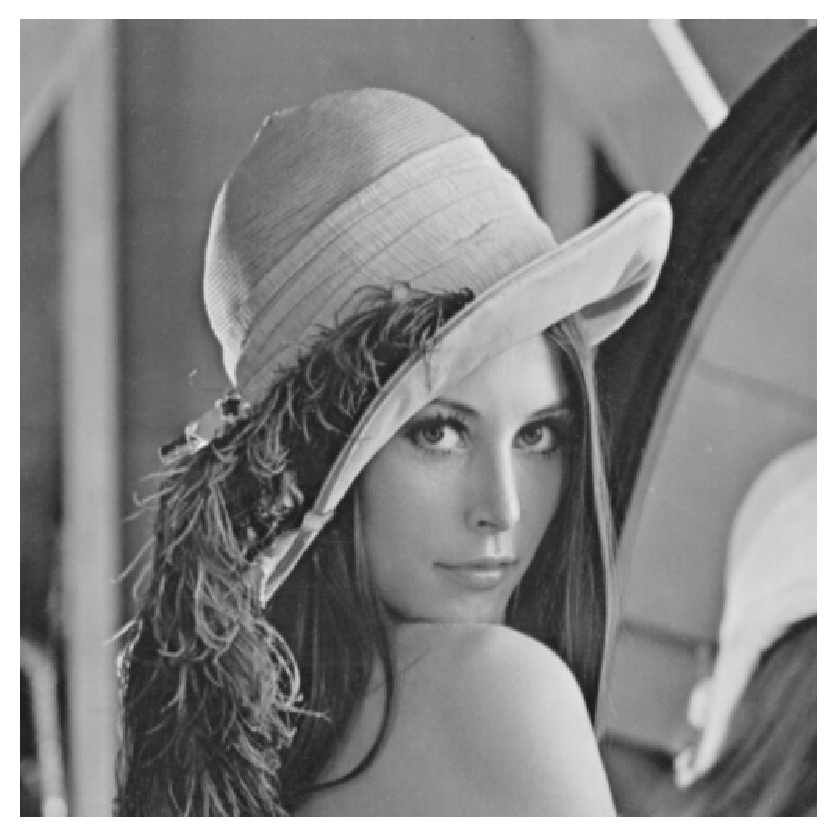
\includegraphics[width=1.3in]{./Figures/Lena/Trad_EF.eps}
  \end{minipage}%
  }% This is important! use % to indicate same line, otherwise new line
  \subfigure[229MHz,~SNR:20.6dB]{
  \begin{minipage}[c]{0.24\textwidth}
    \centering
    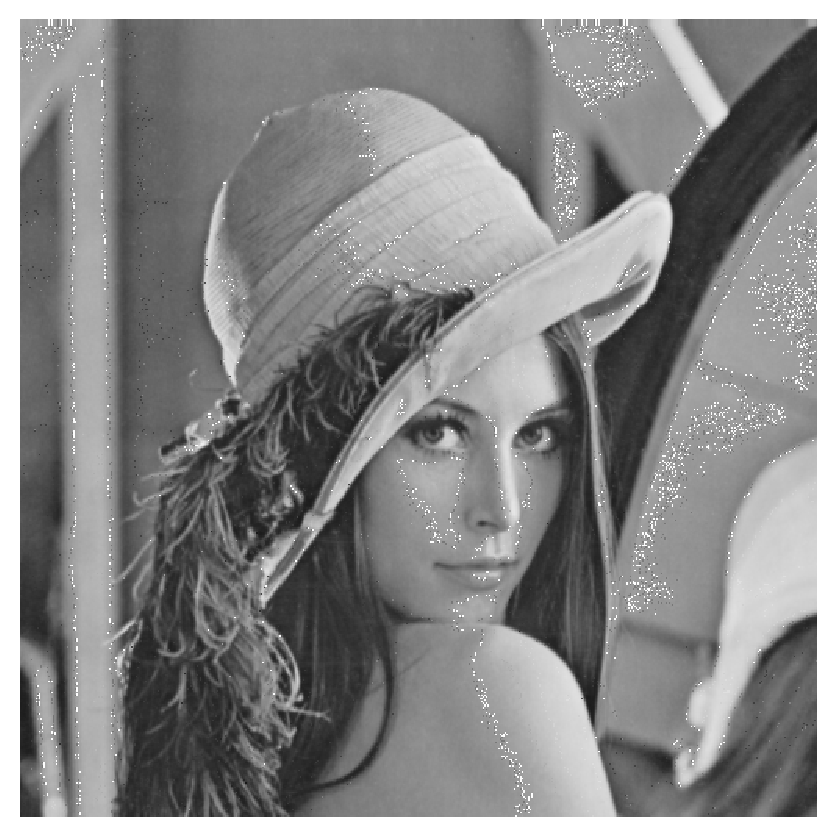
\includegraphics[width=1.3in]{./Figures/Lena/Trad_T436.eps}
  \end{minipage}
  }\vspace{-1ex}
  \subfigure[242MHz,~SNR:38.3dB]{
  \begin{minipage}[c]{0.24\textwidth}
    \centering
    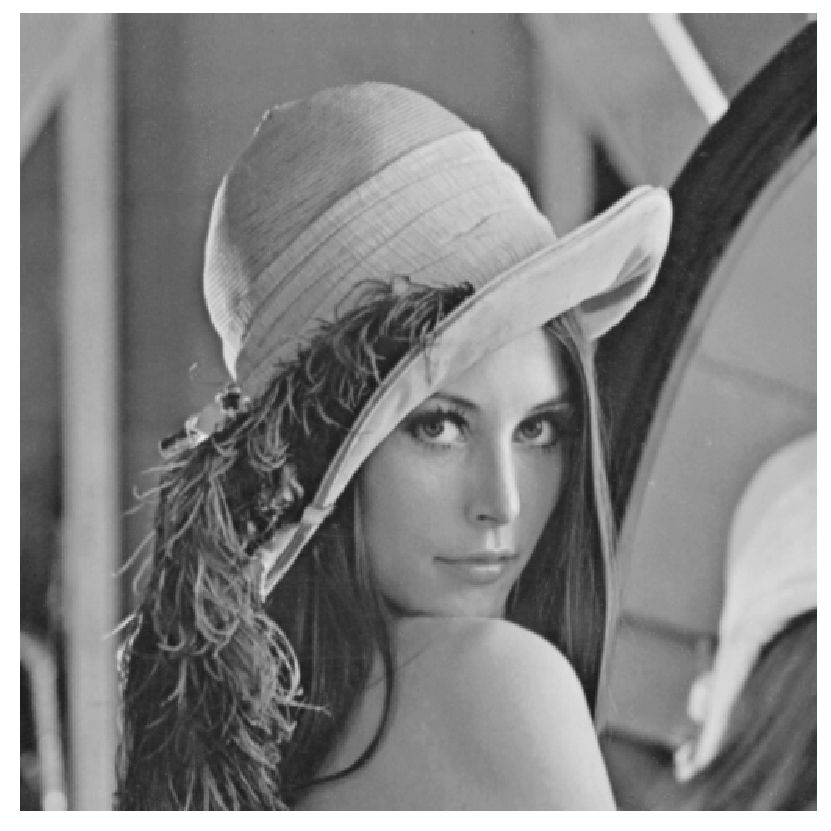
\includegraphics[width=1.3in]{./Figures/Lena/Online_T436.eps}
  \end{minipage}
  }%
  \subfigure[242MHz,~SNR:15.6dB]{
  \begin{minipage}[c]{0.24\textwidth}
    \centering
    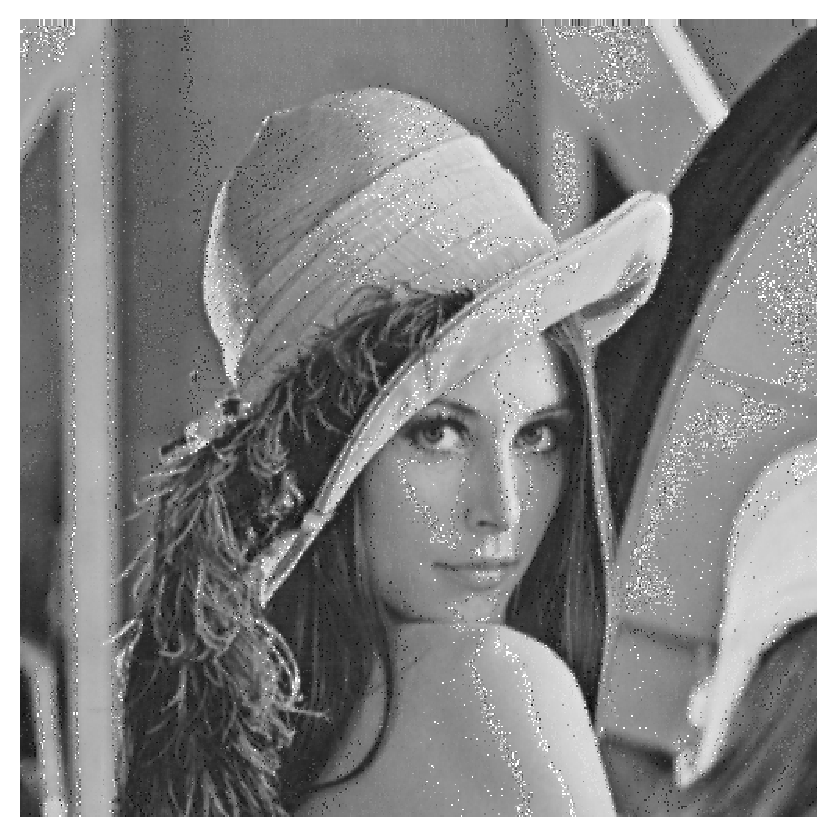
\includegraphics[width=1.3in]{./Figures/Lena/Trad_T414.eps}
  \end{minipage}
  }\vspace{-1ex}
  \subfigure[250MHz,~SNR:36.2dB]{
  \begin{minipage}[c]{0.24\textwidth}
    \centering
    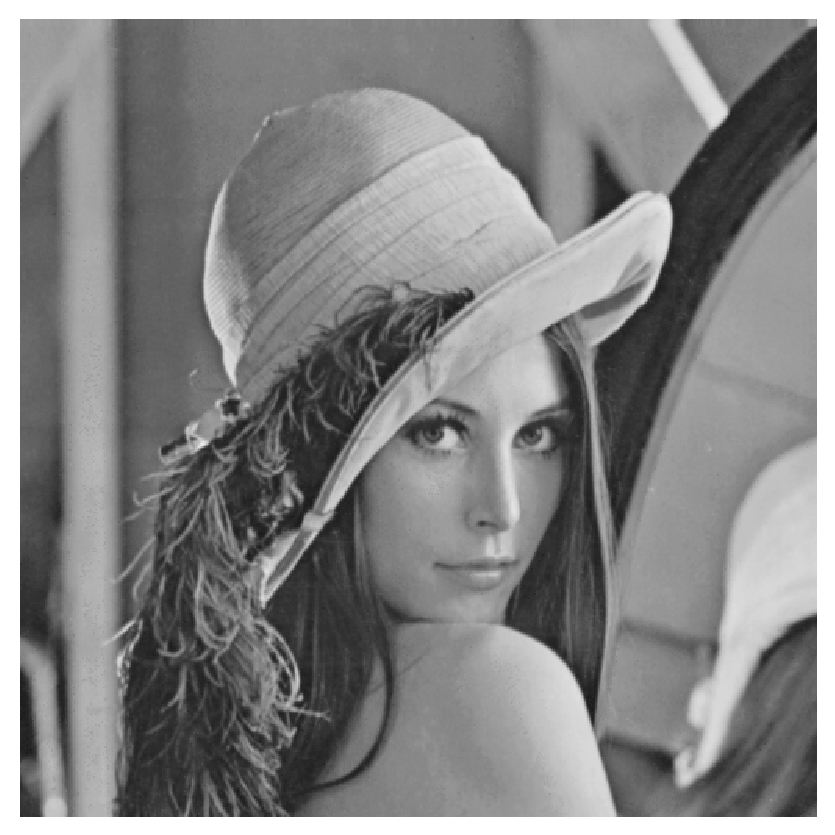
\includegraphics[width=1.3in]{./Figures/Lena/Online_T414.eps}
  \end{minipage}%
  }% same line
  \subfigure[250MHz,~SNR:8.5dB]{
  \begin{minipage}[c]{0.24\textwidth}
    \centering
    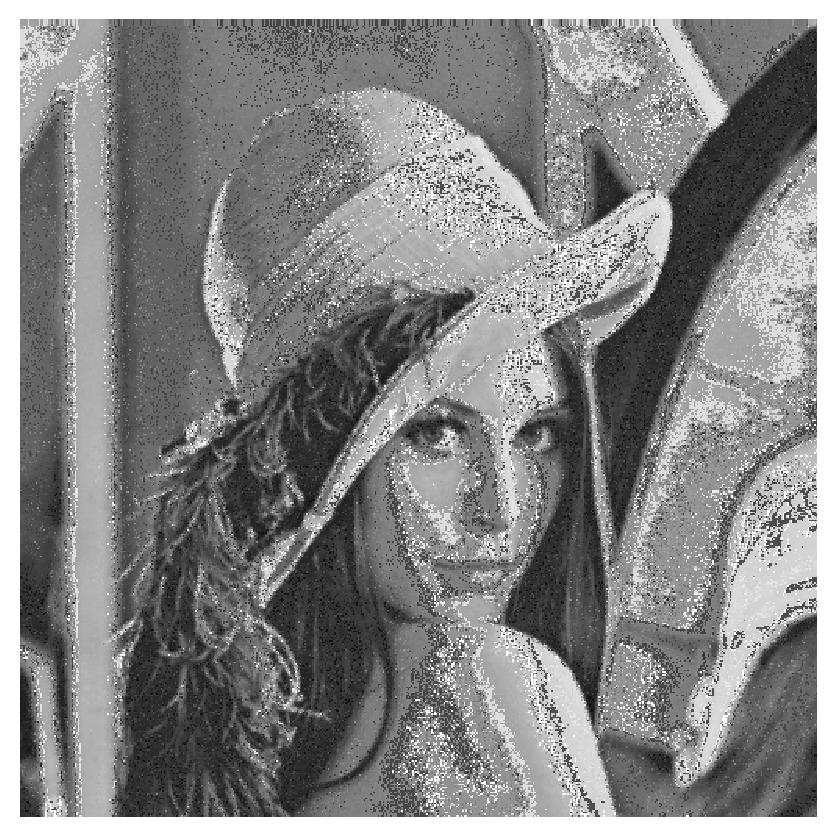
\includegraphics[width=1.3in]{./Figures/Lena/Trad_T400.eps}
  \end{minipage}
  }
\vspace{-2ex}
\caption{Output images of image filter using online arithmetic (left column) and traditional arithmetic (right column).}
\label{Fig:LenaImage}
\vspace{-2ex}
\end{figure}

\subsection{Potential Benefits in Circuit Design}
In general, our results could be of interest to a circuit design in two folds. Typically by choosing different computing arithmetics and data representations, either a circuit can be designed to operate at a certain frequency with the minimum possible MRE, or a given error budget specified by the algorithm designer can be met with the fastest achievable operating frequency. For the first case, the experimental results obtained by uniform independent inputs together with 4 benchmark images are summarized in Table xxx in terms of the difference of SNR and the relative reduction of MRE as given by () where $MRE_{OL}$ and $MRE_{Trad}$ denote the value obtained with online arithmetic and with traditional arithmetic, respectively.
%
\begin{eqnarray}
  \frac{MRE_{Trad}-MRE_{OL}}{MRE_{Trad}}\times100\%
\end{eqnarray}
%
For a fairer comparison, the frequency in this table is normalized to the maximum error-free frequency for each arithmetic. It can be seen that a significant reduction of MRE can be obtained using online arithmetic for all input types. The geometric mean reduction varies from $97.3\%$ to $98.2\%$. In addition, larger differences of MRE reduction can be achieved in practice. This is because long chains occur with even smaller probabilities with real data. Similarly from Table xxx, the differences in SNR vary from 21.4dB to 43.9dB.

\begin{table}[tbp]
\renewcommand{\arraystretch}{1.1}
\setlength{\tabcolsep}{4.1pt}
\caption{Relative Reduction of MRE with Online Arithmetic for Various Normalized Frequencies.}
\small
\centering
\begin{tabular}{|c|ccccc|c|}
\hline
\multirow{2}*{\textbf{Inputs}} & \multicolumn{5}{c|}{\textbf{Normalized Frequency}} &
\multirow{2}*{\begin{tabular}{c}\textbf{Geo.}\\\textbf{Mean}\end{tabular}}\\
& 1.05 & 1.10 & 1.15 & 1.20 & 1.25 &\\
\hline
Uniform & 94.5\% & 89.1\% & 90.1\% & 88.3\% & 84.3\% & 89.2\%\\
Lena    & 99.3\% & 99.2\% & 98.9\% & 97.7\% & 94.9\% & 97.9\%\\
Pepper  & 99.7\% & 98.3\% & 98.1\% & 97.2\% & 95.1\% & 97.7\%\\
Sailboat& 99.5\% & 97.9\% & 97.3\% & 96.8\% & 95.1\% & 97.3\%\\
Tiffany & 99.9\% & 97.6\% & 98.4\% & 97.8\% & 97.2\% & 98.2\%\\
\hline
\end{tabular}
\label{Tab:}
\vspace{-2ex}
\normalsize
\end{table}

\begin{table}[tbp]
\renewcommand{\arraystretch}{1.1}
\setlength{\tabcolsep}{4.1pt}
\caption{Improvement of SNR with Online Arithmetic for Various Normalized Frequencies}
\small
\centering
\begin{tabular}{|c|ccccc|}
\hline
\multirow{2}*{\textbf{Inputs}} & \multicolumn{5}{c|}{\textbf{Normalized Frequency}} \\
& 1.05 & 1.10 & 1.15 & 1.20 & 1.25\\
\hline
Lena    & 44.6 & 36.3 & 33.2 & 29.1 & 22.9\\
Pepper  & 35.7 & 28.3 & 28.7 & 25.9 & 24.1\\
Sailboat& 33.7 & 27.5 & 26.3 & 25.0 & 21.7\\
Tiffany & 43.9 & 25.9 & 29.5 & 25.6 & 24.5\\
\hline
\end{tabular}
\label{Tab:}
\vspace{-2ex}
\normalsize
\end{table}


\begin{table}[tbp]
\renewcommand{\arraystretch}{1.1}
\setlength{\tabcolsep}{4.1pt}
\caption{Relative Reduction of MRE with Online Arithmetic for Various Normalized Frequencies.}
\small
\centering
\begin{tabular}{|c|cccc|c|}
\hline
\multirow{2}*{\textbf{Inputs}} & \multicolumn{4}{c|}{\textbf{Normalized Frequency}} &
\multirow{2}*{\begin{tabular}{c}\textbf{Geo.}\\\textbf{Mean}\end{tabular}}\\
& 0.01\% & 0.1\% & 1\% & 10\% &\\
\hline
Uniform & N/A & 4.59\%   & 8.78\%  & 12.83\% & 8.03\%\\
Lena    & 7.96\% & 11.50\%  & 16.39\% & 13.71\% & 11.88\%\\
Pepper  & 6.22\% & 8.87\%   & 18.68\% & 15.94\% & 11.32\%\\
Sailboat& 5.71\% & 8.87\%   & 16.93\% & 15.29\% & 10.70\%\\
Tiffany & 2.35\% & 6.90\%   & 18.58\% & 12.22\% & 7.79\% \\
\hline
\end{tabular}
\label{Tab:}
\vspace{-2ex}
\normalsize
\end{table}

%\end{document}  % This is where a 'short' article might terminate

%ACKNOWLEDGMENTS are optional
%\section{Acknowledgments}
%This section is optional;
%
% The following two commands are all you need in the
% initial runs of your .tex file to
% produce the bibliography for the citations in your paper.
\bibliographystyle{abbrv}
\bibliography{Reference}  % sigproc.bib is the name of the Bibliography in this case
%  and remember to run:
% latex bibtex latex latex
% to resolve all references
%

\end{document}
